\scanpage{62}
\mspage{18}
One should make explicit a \uline{small} preliminary dévissage theorem, which \unsure{says|will say} that up to equivalence (defined up to \unsure{unique|unique} isomorphism)
$S_{\unsure{*|f}}\mathcal TD_{\mathrm{top}}^\pm$,
\inserted{\unsure{with|over} the functor $\Gamma$ to $(\mathrm{Gr.pond\ top})$ and $\unsure{\chi|f}$ to $[\pm1]$, and}
with the elementary operations $1^\circ:7^\circ$
\margin{\uline{with the exception}\\\uline{of $4^\circ$ and $5^\circ$}}
(or their\unsure{s|\deleted{s}} simultaneous composite \unsure{variant|variants}) is reconstructed from knowledge of the following groupoids and functors

\diagram{\deleted{\mbox{\begin{tikzcd}[ampersand replacement=\&,row sep=large,column sep=large]
S_1\mathcal T_{g,\nu}^{\deleted{\unsure{0|\infty}}\pm}\arrow[r,"{\unsure{\chi}}"]\arrow[d]
\&{[\pm1]}\\
\mathrm{Ens}(\nu)
\end{tikzcd}}}}
\diagram{\deleted{\mbox{\begin{tikzcd}[ampersand replacement=\&,row sep=large]
\&\mathcal T_{g,\nu}^{\pm}\arrow[dl]\\
{}\&
\end{tikzcd}}}}

\diagram{\begin{tikzpicture}
\node[inner sep=9pt] (live) {\begin{tikzcd}[ampersand replacement=\&,column sep=large]
S_1\mathcal T_{g,\nu}^\pm\arrow[r]
\&\mathcal T_{g,\nu}^\pm\arrow[r]
\&(\mathrm{Ens}(\nu)\times[\pm1])
\end{tikzcd}};
\draw (live.north west)--(live.north east);
\draw (live.south west)--(live.south east);
\draw ([yshift=-3pt]live.north west)--([yshift=3pt]live.south west);
\node[anchor=east] at ([xshift=-3pt]live.west) {$(*)$};
\node[anchor=north west,align=left,font=\footnotesize] (short)
 at ([xshift=20pt,yshift=-10pt]live.south west)
 {we shall abbreviate as\\$S\mathcal T_{g\nu}^{\pm}$};
\draw ([xshift=15pt,yshift=11pt]live.south west)
 to[out=-95,in=145] ([xshift=-2pt]short.west);
\node[anchor=south,inner sep=0pt]
 at ([xshift=-2.3cm]live.south east) {$\deleted{\unsure{E|\mathrm{En}|\varnothing}}$};
\end{tikzpicture}}
\margin{This is not quite enough, to have all the operations
In particular the operations \textcircled{$4^\circ$} (which \unsure{requires|changes}
\deleted{\unsure{the introduction|links}} \inserted{\unsure{``or''}} of the
``structures'' $\mathcal T_{g,\unsure{\infty|\nu}}$) and \textcircled{$5^\circ$}}

$S_1\mathcal T_{g,\nu}^\pm$ denotes the subgroupoid of $S_*\mathcal T_{\mathrm{top}}^\pm$ consisting of the $(X,R)$ such that $X$ is connected of genus $g$, $\operatorname{card}\pi_0\partial X=\nu$, and $\operatorname{card}R\cap C_{\unsure{-|a|\cdot}}=1$ (for every $a\in\pi_0\partial X$ --- i.e. the \inserted{doubly weighted} graph of the
$\deleted{\mathcal T_{g,\nu}}(X,\underset{\substack{\Vert\\\partial X}}{\widetilde\Sigma},R)$ is isomorphic to
\figure{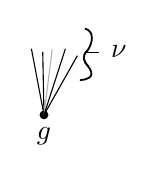
\begin{tikzpicture}[scale=.8]
\fill (0,0) circle(2pt);
\node[below] at (0,-.04) {$g$};
\draw (0,0)--(-.20,1.05);
\draw (0,0)--(-.02,1.00);
\draw[gray!60] (0,0)--(.13,1.04);
\draw (0,0)--(.34,1.05);
\draw (0,0)--(.53,.94);
\draw[line width=.65pt] (.65,1.37)
 .. controls (.80,1.33) and (.78,1.15) .. (.69,1.02)
 .. controls (.60,.94) and (.62,.85) .. (.70,.77)
 .. controls (.80,.64) and (.76,.57) .. (.57,.55);
\draw[line width=.65pt] (.66,.99)--(.87,.99);
\draw[line width=.45pt] (.69,1.03)
 .. controls (.59,.94) and (.64,.84) .. (.71,.77);
\node[right] at (.91,1.00) {$\nu$};
\end{tikzpicture}}
all these edges (free) are of weight $1$

and $\mathcal T_{g,\nu}^\pm$ is defined correspondingly, via the $(X,\phi,\phi)$ where $X$ of type $g,\nu$.
\mspage{61}
